\documentclass[british,titlepage, oneside]{ntnuthesis}

\title{An NTNU Thesis \LaTeX{} Document Class}
\shorttitle{An NTNU Thesis Document Class}
\author{Community of Practice in Computer Science Education at NTNU}
\shortauthor{CoPCSE$@$NTNU}
\date{CC-BY \ntnuthesisdate}

\addbibresource{thesis.bib}

\makeglossaries

\setabbreviationstyle[acronym]{long-postshort-user}
\glssetcategoryattribute{acronym}{nohyperfirst}{true}
\setabbreviationstyle{short-nolong}

\newglossaryentry{asyncio}{name=thing,description={A Python library for asynchronous code using coroutines, event loops, and tasks.}}
% --------------------
% ----- Acronyms -----
% --------------------

\newacronym{nvs}{NVS}{Novel View Synthesis}
\newacronym{mlp}{MLP}{Multi-Layer Perceptron}
\newacronym{nerf}{NeRF}{Neural Radiance Field}
\newacronym{rt}{RT}{Ray Tracing}
\newacronym{bvh}{BVH}{Bounding Volume Hierarchy}

% \glsaddall
% \glsunset{cpu}
% \glsunset{gpu}
% \glsunset{lla}
% --------------------
% ----- Shortcuts ----
% --------------------


\newcommand{\nvidia}{NVIDIA\xspace}

\newcommand{\jetson}{\gls{jetson}\xspace}
\newcommand{\sr}{Sensor Rig\xspace}
\newcommand{\jx}{Xavier\xspace}
\newcommand{\jo}{Orin\xspace}
\newcommand{\gs}{Gstreamer\xspace}
\newcommand{\cam}{Triton Polarizin Camera\xspace}
\newcommand{\cams}{Triton Polarizin Cameras\xspace}
\newcommand{\lucid}{Lucid Vision\xspace}
\newcommand{\preproject}{Pre-Project\xspace}
\newcommand{\master}{Master's\xspace}
\newcommand{\py}{Python\xspace}
\newcommand{\cpu}{\gls{gpu}\xspace}
\newcommand{\gpu}{\gls{cpu}\xspace}
\newcommand{\gui}{GUI\xspace}
\newcommand{\guif}{\gls{gui} framework\xspace}
\newcommand{\srgui}{\sr \gls{gui}\xspace}
 % add glossary and acronym lists before document
% \oneside

\begin{document}

\chapter*{Abstract}

The \texttt{ntnuthesis} document class is a customised version of the standard \LaTeX{} \texttt{report} document class. It can be used for theses at all levels – bachelor, master and PhD – and is available in English (British and American) and Norwegian (Bokmål and Nynorsk). This document is ment to serve (i) as a description of the document class, (ii) as an example of how to use it, and (iii) as a thesis template.

\chapter*{Sammendrag}

Dokumentklassen \texttt{ntnuthesis} er en tilpasset versjon av \LaTeX' standard \texttt{report}-klasse. Den er tilrettelagt for avhandlinger på alle nivåer – bachelor, master og PhD – og er tilgjengelig på både norsk (bokmål og nynorsk) og engelsk (britisk og amerikansk). Dette dokumentet er ment å tjene (i) som en beskrivelse av dokument\-klassen, (ii) som et eksempel på bruken av den, og (iii) som en mal for avhandlingen.


\tableofcontents
\listoffigures
\listoftables
\lstlistoflistings

\printglossary[type=\acronymtype] % Print acronyms
\printglossary                    % Print glossary

\chapter{Introduction}

Over the years, several thesis templates for \LaTeX{} have been developed by different groups at NTNU. Typically, there have been local templates for given study programmes, or different templates for the different study levels – bachelor, master, and \acrshort{phd}.\footnote{see, e.g., \url{https://github.com/COPCSE-NTNU/bachelor-thesis-NTNU} and \url{https://github.com/COPCSE-NTNU/master-theses-NTNU}}

Based on this experience, the \acrfull{CoPCSE}\footnote{\url{https://www.ntnu.no/wiki/display/copcse/Community+of+Practice+in+Computer+Science+Education+Home}} is hereby offering a template that should in principle be applicable for theses at all study levels. It is closely based on the standard \LaTeX{} \texttt{report} document class as well as previous thesis templates. Since the central regulations for thesis design have been relaxed – at least for some of the historical university colleges now part of NTNU – the template has been simlified and put closer to the default \LaTeX{} look and feel.

The purpose of the present document is threefold. It should serve (i) as a description of the document class, (ii) as an example of how to use it, and (iii) as a thesis template.

\chapter{Using the Document Class}
\label{chap:usage}

\section{Thesis Setup and Language Selection}
\label{sec:setup}

The document class is initialized by issuing the \texttt{\textbackslash documentclass[]\{ntnuthesis\}} at the beginning of your \texttt{.tex} file. The thesis language should be given as an option. Currently British English (class option \texttt{[british]}), American English (class option \texttt{[american]}), Norwegian Bokmål (class option \texttt{[norsk]}) and Norwegian Nynorsk (class option \texttt{[nynorsk]}) are supported.\footnote{Disclaimer: this unfortunate naming of the Norwegian language options follows from the naming conventions of the \texttt{babel} package.}

There is also the \texttt{titlepage} class option that triggers the generation of a simple title page that can be used as a placeholder when writing the thesis. This option should be removed before handing in the thesis. Instead the official NTNU titlepage for the corresponding thesis type should be added as described on Innsida.\footnote{see \url{https://innsida.ntnu.no/wiki/-/wiki/English/Finalizing+the+bachelor+and+master+thesis} for bachelor and master, and \url{https://innsida.ntnu.no/wiki/-/wiki/English/Printing+your+thesis} for PhD.}

\section{Title, Author, and Date}

In the preample of the \texttt{.tex} file, the thesis title should be set with the \texttt{\textbackslash title\{\}} command. The title will appear on the titlepage as well as in the running header of the even numbered pages. If the title is too long for the header, you can use \texttt{\textbackslash shorttitle\{\}} to set a version for the header.

The authors should be listed with full names in the \texttt{\textbackslash author\{\}} command. If there are several authors, they should be separated with \texttt{\textbackslash and}, e.g., like this: \texttt{\textbackslash author\{Anne Andersen \textbackslash and Bjørn Bjørnsen\}}. For the running headers, you may want to use \texttt{\textbackslash shortauthor}, e.g. like this: \texttt{\textbackslash shortauthor\{A. Andersen and B. Bjørnsen\}} or even \texttt{\textbackslash shortauthor\{Andersen et al.\}}.

Use \texttt{\textbackslash date\{\}} to set the date of the document. It will only  appear on the temporary title page. To keep track of temporary versions, it can be a good idea to use \texttt{\textbackslash date\{\textbackslash today\}} while working on the thesis. You may also add copyright and licence information in this field.

\section{Page Layout}

The document class is designed to work with twosided printing. This means that all chapters start on odd (right hand) pages, and that blank pages are inserted where needed to make sure this happens. However, since the theses are very often read on displays, the margins are kept the same on even and odd pages in order to avoid that the page is jumping back and forth upon reading.

To avoid blank pages when rendering the thesis, you can enable the \texttt{oneside} option in the \texttt{thesis.tex} file. Just add 'oneside' to the document class options on the first line, and recompile.

\section{Structuring Elements}

The standard \LaTeX{} elements for document structure are supported: chapter, section, and:

\subsection{This is a \texttt{\textbackslash subsection\{\}}}

Short subsection text here.

\subsubsection{This is a \texttt{\textbackslash subsubsection\{\}}}

Short subsubsection text here.

\paragraph{This is a \texttt{\textbackslash paragraph\{\}}}

Short paragraph text here.

Chapters, sections, and subsections will be included in the table of contents, whereas the lower level structuring elements will not appear there. Don't use too many levels of headings; how many are appropriate, will depend on the size of the document. Also, don't use headings too frequently.

Make sure that the chapter and section headings are correctly capitalised depending on the language of the thesis, e.g., `\emph{Correct Capitalisation of Titles in English}' vs. `\emph{Korrekt staving av titler på norsk}'.

Simple paragraphs are the lowest structuring elements and should be used the most. They are made by leaving one (or more) blank line(s) in the \texttt{.tex} file. In the typeset document they will appear indented and with no vertical space between them.

\section{Lists}

Numbered and unnumbered lists, i.e., the \texttt{enumerate} and \texttt{itemize} environments, are used just as in regular \LaTeX{}, but are typeset somewhat more densely and with other labels. Unnumbered list:
\begin{itemize}
  \item first item
  \item second item
        \begin{itemize}
          \item first subitem
          \item second subitem
                \begin{itemize}
                  \item first subsubitem
                  \item second subsubitem
                \end{itemize}
        \end{itemize}
  \item last item
\end{itemize}
Numbered list:
\begin{enumerate}
  \item first item
  \item second item
        \begin{enumerate}
          \item first subitem
          \item second subitem
                \begin{enumerate}
                  \item first subsubitem
                  \item second subsubitem
                \end{enumerate}
        \end{enumerate}
  \item last item
\end{enumerate}

For description lists, see usage in, e.g., \cref{sec:frontmatter}.

\section{Figures}

Figures are placed in the \texttt{figure} environment. An example is shown in \cref{fig:mapNTNU}. Figures are floats, hence they will float freely around in the document in accordance with standard \LaTeX{} behaviour. You may want to try to override \LaTeX{}'s default placement by using the \texttt{h} (here), \texttt{t} (top of page), \texttt{b} (bottom of page), and \texttt{p} (separate page) options in order of priority. If you provide an alternate (typically shorter) caption in square brackets, it will be used in the list of figures. Use \texttt{\textbackslash includegraphics[]\{\}} with options \texttt{scale} or \texttt{width} to include the graphics file. The caption should be placed \emph{below} the figure. If the caption consists of a single sentence fragment (incomplete sentence), it should not be punctuated. Given the shape and size of the figure, the figure caption can appear too close or too far from the figure. To deal with this, vertical space, either positive or negative, can be added before and/or after the caption command using the \texttt{\textbackslash vspace{}} command.

\begin{figure}[htbp]  % order of priority: h here, t top, b bottom, p page
  \centering
  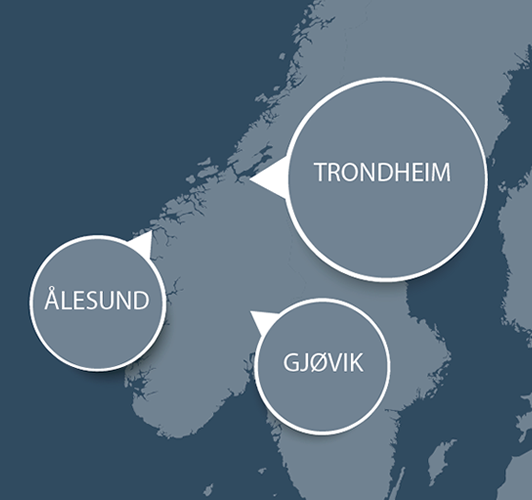
\includegraphics[width=.5\textwidth]{figures/kart_student}
  \caption[Map of NTNU Campuses]{The map shows the three main campuses of NTNU.}
  \label{fig:mapNTNU}
\end{figure}

For figures compsed of several sub-figures, the \texttt{caption} and \texttt{subcaption} packages have been preloaded. See \cref{fig:subfig} with \cref{sfig:a,sfig:b} for an example. For more details on alignment etc., see the Overleaf documentation.\footnote{\url{https://www.overleaf.com/learn/latex/How_to_Write_a_Thesis_in_LaTeX_(Part_3):_Figures,_Subfigures_and_Tables}}

\begin{figure}
  \centering
  \begin{subfigure}[b]{.45\textwidth}
    \centering
    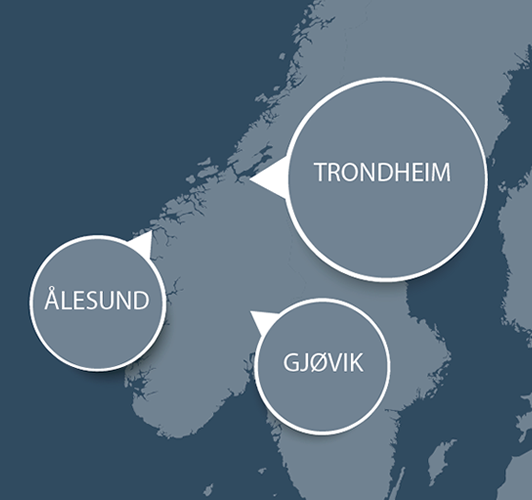
\includegraphics[width=\textwidth]{figures/kart_student.png}
    \caption{First sub-figure}
    \label{sfig:a}
  \end{subfigure}
  \hfill
  \begin{subfigure}[b]{.45\textwidth}
    \centering
    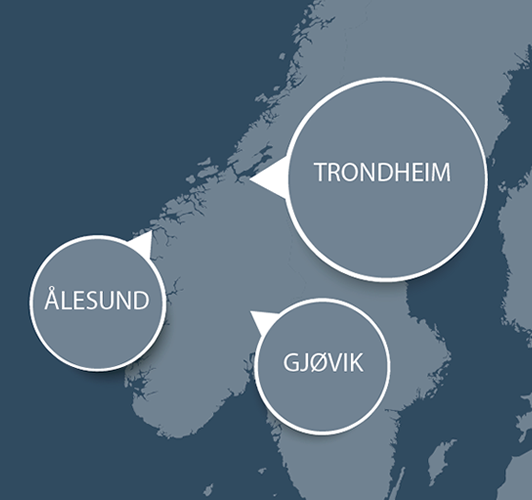
\includegraphics[width=\textwidth]{figures/kart_student.png}
    \caption{Second sub-figure}
    \label{sfig:b}
  \end{subfigure}
  \caption{A figure composed of two sub-figures. It has a long caption in order to demonstrate how that is typeset.}
  \label{fig:subfig}
\end{figure}

You can make nice graphs directly from data files using \texttt{gnuplot}, but it is expensive on every compilation.  The code is included in the
raw latex as a comment so you can uncomment that code to see how it works.
% , for an example, see \cref{fig:examplegnuplot}.
%
%\begin{figure}[htbp]
%  \centering
%    \begin{gnuplot}[terminal=epslatex,terminaloptions={size 8cm,6cm color}]
%        set xlabel "age"
%        set ylabel "IQ"
%        set key autotitle columnhead
%        set title "age vs IQ"
%        set yrange [0:160]
%        set datafile separator ","
%        plot "csvtables/ageiq.csv" using 1:2 with boxes
%    \end{gnuplot}
%  \caption[An example of Integrated Graph]{This is a gnuplot graph read from a file. Also this figure has a long caption in order to demonstrate how that is typeset.}
%  \label{fig:examplegnuplot}
%\end{figure}

\section{Tables}

Tables are placed in the \texttt{table} environment. An example is given in \cref{tab:example1}. Like figures, tables float freely around in the document in accordance with standard \LaTeX{} behaviour. The table caption should be placed \emph{above} the table. If the caption consists of a single sentence fragment (incomplete sentence), it should not be punctuated.

\begin{table}
  \centering
  \caption{A simple, manually formatted example table}
  \label{tab:example1}
  \begin{tabular}{cc}
    \hline
    age & IQ  \\
    \hline
    10  & 110 \\
    20  & 120 \\
    30  & 145 \\
    40  & 120 \\
    50  & 100 \\
    \hline
  \end{tabular}
\end{table}

Tables can also be automatically generated from CSV files using the \texttt{simplecsv} and \texttt{booktab} packages. See \cref{tab:examplecsv} for an example.

\begin{table}[tbp]
  \centering
  \caption[A simple example table generated from a CSV file]{A simple example table generated from a CSV file using \texttt{simplecsv} and \texttt{booktab}}
  \label{tab:examplecsv}
  \csvautobooktabular{csvtables/ageiq.csv}
\end{table}

\section{Listings}

Code listings are included by means of the \texttt{listings} package. Code examples can be read from file or provided inline, and should be given a caption for cross referencing and for appearance in the list of code listings in the thesis frontmatter. If all your code examples are written in the same programming language, you can use, e.g., \texttt{\textbackslash lstset\{language=Python\}} to set the language once and for all. The code is set with the monospace font, and the font size is reduced to allow for code lines up to at least 80 characters without causing line breaks. Options for programming languages, line numbering etc. are provided. Unlike figures and tables, code listings are not floating objects, and will appear at the same position in the typeset document as in the \texttt{.tex} file. If the caption consists of a single sentence fragment (incomplete sentence), it should not be punctuated.

\lstinputlisting[
  caption={Python example from file},
  label=lst:pythonfile,
  language=Python
]{listings/example.py}

\lstinputlisting[%
  caption={C++ example from file},
  label=lst:cppfile,
  language=C++,
  numbers=left
]{listings/example.cc}

\begin{lstlisting}[
    caption={Python code in \LaTeX{} document},
    label=lst:pythondoc,
    language=Python]
import numpy as np
import matplotlib.pyplot as plt

x = np.linspace(0, 1)
y = np.sin(2 * np.pi * x)

plt.plot(x, y)
plt.show()
\end{lstlisting}

\begin{lstlisting}[
    caption={C++ code in \LaTeX{} document},
    label=lst:cppdoc,
    language=C++]
#include <iostream>
using namespace std;

int main()
{
  cout << "Hello, World!" << endl;
  return 0;
}
\end{lstlisting}

\section{Equations}

Equations are typeset as normally in \LaTeX{}. It is common to consider equations part of the surrounding sentences, and include punctuation in the equations accordingly, e.g.,
\begin{equation}
  f(x) = \int_1^x \frac{1}{y}\,dy = \ln x\,.
  \label{eq:logarithm}
\end{equation}
For more advanced symbols like, e.g., $\mathbb{R}, \mathbb{Q}$, the \texttt{amssymb} package is preloaded, and for more advanced mathematical layout the \texttt{amsmath} behaviour is obtained through the \texttt{mathdesign} package. Confer the overleaf documentation for details.\footnote{\url{https://www.overleaf.com/learn/latex/Mathematical_expressions}}

\section{Fonts}

Bitstream Charter at 11pt with the corresponding Mathdesign math fonts have been selected as the main fonts for the thesis template. For code examples, the monospaced font should be used – for this, a scaled version of the DejaVuSansMono to match the main font is preselected. If you would like to use an accompanying sans serif font, the BeraSans has been made available. The standard \LaTeX{} font commands should be used to switch between fonts, e.g.,
\texttt{\textbackslash textit\{\}} \textit{for italics},
\texttt{\textbackslash textbf\{\}} \textbf{for bold face},
\texttt{\textbackslash texttt\{\}} \texttt{for mono spaced}, and
\texttt{\textbackslash textsf\{\}} \textsf{for sans serif}.
For generic \emph{emphasis}, \texttt{\textbackslash emph\{\}} should be applied.

\section{Cross References}
\label{sec:crossref}

For cross references, i.e., references within the document, the \texttt{\textbackslash cref\{\}} command provided byt the \texttt{cleveref} package should be used. Labels are inserted in the document in the standard \LaTeX{} manner. They are case sensitive, so, e.g., a label immediately after a section command refers to that section, while a label within, e.g., a table environment refers to the table. The \texttt{\textbackslash cref\{\}} command also generates the corresponding text. If the document is in English (class options \texttt{british} or \texttt{american}), the cross references are capitalised, whereas if it is in Norwegian (class options \texttt{norsk} or \texttt{nynorsk}), they are not. If you are writing in Norwegian, you should use \texttt{\textbackslash Cref\{\}} at the beginning of a sentence to ensure that the cross reference is correctly capitalised. For examples on usage, see \cref{sec:crossref} in \cref{chap:usage}, \cref{tab:example1}, \cref{fig:mapNTNU}, \cref{eq:logarithm}, \cref{lst:cppfile}, \cref{paper:scrutiny}, and \cref{app:additional}. \Cref{app:additional} at the beginning of a sentence.

The cross references are made into active hyperlinks in the resulting PDF document by the use of the \texttt{hyperref} package. The colour of the links is set to black for best appearance on print. This can easily be changed by the author by the use of the \texttt{\textbackslash hypersetup\{\}} command.

\section{Glossary and Acronyms}
The template comes with the ability to create a glossary and acronym list. To add entries to one of these lists, add them to the \texttt{glossary.tex} file.
All uses of the acronym and glossary functions will create a clickable link that references the corresponding entry in one of the lists. All entries in the lists will also contain page references to all places it has been used.
\subsection{Using Acronyms}
To render acronyms, you have three options:
\begin{itemize}
  \item \texttt{\textbackslash acrlong\{ \}} prints the phrase the acronym stands for, e.g. \texttt{\textbackslash acrlong\{gcd\}} displays \acrlong{gcd}.
  \item \texttt{\textbackslash acrshort\{ \}} prints the acronym, e.g. \texttt{\textbackslash acrshort\{gcd\}} displays \acrshort{gcd}.
  \item \texttt{\textbackslash acrfull\{ \}} prints both the acronym and its definition, e.g. \texttt{\textbackslash acrfull\{gcd\}} displays \acrfull{gcd}.
\end{itemize}

\subsection{Using Glossary}
\begin{itemize}
  \item \texttt{\textbackslash gls\{ \}} prints the term in lowercase, e.g. \texttt{\textbackslash gls\{maths\}} displays \gls{maths}.
  \item \texttt{\textbackslash Gls\{ \}} prints the term in with first letter in uppercase, e.g. \texttt{\textbackslash Gls\{maths\}} displays \Gls{maths}.
  \item \texttt{\textbackslash glspl\{ \}} prints the term in plural form, e.g. \texttt{\textbackslash glspl\{bibliography\}} displays \glspl{bibliography}.
  \item \texttt{\textbackslash Glspl\{ \}} prints the term in plural form capitalized, e.g. \texttt{\textbackslash Glspl\{bibliography\}} displays \Glspl{bibliography}.
\end{itemize}


\section{Bibliography}

The \gls{bibliography} is typset using the \texttt{biblatex} package with the \texttt{biber} backend. The default citation style is \texttt{numeric-comp}, and the default bibliography style is \texttt{numeric}. This produces a bibliography similar to, but not completely according to, the so-called Vancouver style. With this setup, a single \texttt{\textbackslash cite\{\}} command will give a number only~\cite{landes1951scrutiny}, and \texttt{\textbackslash textcite\{\}} will give author and number like this: \textcite{landes1951scrutiny}. If you would like to give the full reference of a paper within the thesis, e.g., in a list of included papers, use \texttt{\textbackslash fullcite\{\}} like this: \fullcite{landes1951scrutiny}.

\section{Included Papers}

If you are writing a compiled PhD thesis (and probably only then – see \cref{sec:compiledphd}), you will need to attach the papers containing the main contribution of the thesis. This can be done issuing the \texttt{paper} environment. It takes two arguments: (i) the PDF file, and (ii) a label for cross referencing. See \cref{paper:scrutiny} for an example.

\section{Appendices}

Additional material that does not fit in the main thesis but may still be relevant to share, e.g., raw data from experiments and surveys, code listings, additional plots, pre-project reports, project agreements, contracts, logs etc., can be put in appendices. Simply issue the command \texttt{\textbackslash appendix} in the main \texttt{.tex} file, and then the following chapters made by \texttt{\textbackslash chapter\{\}} become appendices. See \cref{app:additional} for an example.

\chapter{Thesis Structure}

The structure of the thesis, i.e., which chapters and other document elements that should be included, depends on several factors such as the study level (bachelor, master, PhD), the type of project it describes (development, research, investigation, consulting), and the diversity (narrow, broad). Thus, there are no exact rules for how to do it, so whatever follows should be taken as guidelines only.

A thesis, like any book or report, can typically be divided into three parts: front matter, body matter, and back matter. Of these, the body matter is by far the most important one, and also the one that varies the most between thesis types.

\section{Front Matter}
\label{sec:frontmatter}

The front matter is everything that comes before the main part of the thesis. It is common to use roman page numbers for this part to indicate this. The minimum required front matter consists of a title page, abstract(s), and a table of contents. A more complete front matter, in a typical order, is as follows.

\begin{description}
    \item[Title page:] The title page should, at minimum, include the thesis title, authors and a date. A more complete title page would also include the name of the study programme, and possibly the thesis supervisor(s). See \cref{sec:setup}.
    \item[Abstracts:] The abstract should be an extremely condensed version of the thesis. Think one sentence with the main message from each of the chapters of the body matter as a starting point. \textcite{landes1951scrutiny} have given some very nice instructions on how to write a good abstract. A thesis from a Norwegian Univeristy should contain abstracts in both Norwegian and English irrespectively of the thesis language (typically with the thesis language coming first).
    \item[Dedication:] If you wish to dedicate the thesis to someone (increasingly common with increasing study level), you may add a separate page with a dedication here. Since a dedication is a personal statement, no template is given. Design it according to your preference.
    \item[Acknowledgements:] If there is someone who deserves a `thank you', you may add acknowledgements here. If so, make it an unnumbered chapter, i.e., \texttt{\textbackslash chapter*\{Acknowledgements\}}.
    \item[Table of contents:] A table of contents should always be present in a document at the size of a thesis. It is generated automatically using the \texttt{\textbackslash tableofcontents} command. The one generated by this document class also contains the front matter and unnumbered chapters.
    \item[List of figures:] If the thesis contains many figures that the reader might want to refer back to, a list of figures can be included here. It is generated using \texttt{\textbackslash listoffigures}.
    \item[List of tables:] If the thesis contains many tables that the reader might want to refer back to, a list of tables can be included here. It is generated using \texttt{\textbackslash listoftables}.
    \item[List of code listings:] If the thesis contains many code listings that the reader might want to refer back to, a list of code listings can be included here. It is generated using \texttt{\textbackslash lstlistoflistings}.
    \item[Other lists:] If there are other list you would like to include, this would be a good place. Examples could be lists of definitions, theorems, nomenclature, abbreviations, glossary etc. There are no standards for this, but many lists can be generated using the \texttt{description} environment (like, e.g., this list of possible front matter content) within a separate \texttt{\textbackslash chapter*\{\}}.
    \item[Preface or Foreword:] A preface or foreword is a good place to make other personal statements that do not fit whithin the body matter. This could be information about the circumstances of the thesis, your motivation for choosing it, or possibly information about an employer or an external company for which it has been written. Again, use, e.g., \texttt{\textbackslash chapter*\{Preface\}}.
\end{description}

\section{Body Matter}

The body matter consists of the main chapters of the thesis. It starts the Arabic page numbering with page~1. There is a great diversity in the structure chosen for different thesis types. Common to almost all is that the first chapter is an introduction, and that the last one is a conclusion followed by the bibliography.

\subsection{Development Project}
\label{sec:development}

For many bachelor and some master projects in computer science, the main task is to develop something, typically a software prototype, for an `employer' (e.g., an external company or a research group). A thesis describing such a project is typically structured as a software development report whith more or less the following chapters:

\begin{description}
    \item[Introduction:] The introduction of the thesis should take the reader all the way from the big picture and context of the project to the concrete task that has been solved in the thesis. A nice skeleton for a good introduction was given by \textcite{claerbout1991scrutiny}: \emph{review–claim–agenda}. In the review part, the background of the project is covered. This leads up to your claim, which is typically that some entity (software, device) or knowledge (research questions) is missing and sorely needed. The agenda part briefly summarises how your thesis contributes.
    \item[Requirements:] The requirements chapter should lead up to a concrete description of both the functional and non-functional requirements for whatever is to be developed at both a high level (use cases) and lower levels (low level use cases, requirements). If a classical waterfall development process is followed, this chapter is the product of the requirement phase. If a more agile model like, e.g., SCRUM is followed, the requirements will appear through the project as, e.g., the user stories developed in the sprint planning meetings.
    \item[Technical design:] The technical design chapter describes the big picture of the chosen solution. For a software development project, this would typically contain the system arcitechture (client-server, cloud, databases, networking, services etc.); both how it was solved, and, more importantly, why this architecture was chosen.
    \item[Development Process:] In this chapter, you should describe the process that was followed. It should cover the process model, why it was chosen, and how it was implemented, including tools for project management, documentation etc. Depending on how you write the other chapters, there may be good reasons to place this chapters somewhere else in the thesis.
    \item[Implementation:] Here you should describe the more technical details of the solution. Which tools were used (programming languages, libraries, IDEs, APIs, frameworks, etc.). It is a good idea to give some code examples. If class diagrams, database models etc. were not presented in the technical design chapter, they can be included here.
    \item[Deployment:] This chapter should describe how your solution can be deployed on the employer's system. It should include technical details on how to set it up, as well as discussions on choices made concerning scalability, maintenance, etc.
    \item[Testing and user feedback:] This chapter should describe how the system was tested during and after development. This would cover everything from unit testing to user testing; black-box vs. white-box; how it was done, what was learned from the testing, and what impact it had on the product and process.
    \item[Discussion:] Here you should discuss all aspect of your thesis and project. How did the process work? Which choices did you make, and what did you learn from it? What were the pros and cons? What would you have done differently if you were to undertake the same project over again, both in terms of process and product? What are the societal consequences of your work?
    \item[Conclusion:] The conclusion chapter is usually quite short – a paragraph or two – mainly summarising what was achieved in the project. It should answer the \emph{claim} part of the introduction. It should also say something about what comes next (`future work').
    \item[Bibliography:] The bibliography should be a list of quality-assured peer-reviewed published material that you have used throughout the work with your thesis. All items in the bibliography should be referenced in the text. The references should be correctly formatted depending on their type (book, journal article, conference publication, thesis etc.). If \texttt{biblatex} is correctly used as proposed by this template, the formatting will be taken care of automatically. The bibliography should not contain links to arbitrary dynamic web pages where the content is subject to change at any point of time. Such links, if necessary, should rather be included as footnotes throughout the document. The main point of the bibliography is to back up your claims with quality-assured material that future readers will actually be able to retrieve years ahead.
\end{description}

\subsection{Research Project}
\label{sec:resesarch}

For many master and some bachelor projects in computer science, the main task is to gain knew knowledge about something. A thesis describing such a project is typically structed as an extended form of a scientific paper, following the so-called IMRaD (Introduction, Method, Results, and Discussion) model:

\begin{description}
    \item[Introduction:] See \cref{sec:development}.
    \item[Background:] Research projects should always be based on previous research on the same and/or related topics. This should be described as a background to the thesis with adequate bibliographical references. If the material needed is too voluminous to fit nicely in the review part of the introduction, it can be presented in a separate background chapter.
    \item[Method:] The method chapter should describe in detail which activities you undertake to answer the research questions presented in the introduction, and why they were chosen. This includes detailed descriptions of experiments, surveys, computations, data analysis, statistical tests etc.
    \item[Results:] The results chapter should simply present the results of applying the methods presented in the method chapter without further ado. This chapter will typically contain many graphs, tables, etc. Sometimes it is natural to discuss the results as they are presented, combining them into a `Results and Discussion' chapter, but more often they are kept separate.
    \item[Discussion:] See \cref{sec:development}.
    \item[Conclusion:] See \cref{sec:development}.
    \item[Bibliography:] See \cref{sec:development}.
\end{description}

\subsection{Monograph PhD Thesis}
\label{sec:monograph}

Traditionally, it has been common to structure a PhD thesis as a single book – a \emph{monograph}. If the thesis is in the form of one single coherent research project, it can be structured along the lines of \cref{sec:resesarch}. However, for such a big work that a PhD thesis constitutes, the tasks undertaken are often more diverse, and thus more naturally split into several smaller research projects as follows:

\begin{description}
    \item[Introduction:] The introduction would serve the same purpose as for a smaller research project described in \cref{sec:development}, but would normally be somewhat more extensive. The \emph{agenda} part should inform the reader about the structure of the rest of the document, since this may vary significantly between theses.
    \item[Background:] Where as background chapters are not necessarily needed in smaller works, they are almost always need in PhD thesis. They may even be split into several chapters if there are significantly different topics to cover. See \cref{sec:resesarch}.
    \item[Main chapters:] Each main chapter can be structured more or less like a scientific paper. Depending on how much is contained in the introduction and background sections, the individual introduction and background sections can be significantly reduced or even omitted completely.
    \begin{itemize}
        \item (Introduction)
        \item (Background)
        \item Method
        \item Results
        \item Discussion
        \item Conclusion
    \end{itemize}
    \item[Discussion:] In addition to the discussions within each of the individual chapters, the contribution of the thesis \emph{as a whole} should be thoroughly discussed here.
    \item[Conclusion:] In addition to the conclusions of each of the individual chapters, the overall conclusion of the thesis, and how the different parts contribute to it, should be presented here. The conclusion should answer to the research questions set out in the main introduction. See also \cref{sec:development}.
    \item[Bibliography:] See \cref{sec:development}.
\end{description}

\subsection{Compiled PhD Thesis}
\label{sec:compiledphd}

Instead of writing up the PhD thesis as a monograph, compiled PhD theses (also known as stapler theses, sandwich theses, integrated theses, PhD by published work) consisting of reproductions of already published research papers are becoming increasingly common. At least some of the papers should already have been accepted for publication at the time of submission of the thesis, and thus have been through a real quality control by peer review.

\begin{description}
    \item[Introduction:] See \cref{sec:monograph}.
    \item[Background:] See \cref{sec:monograph}.
    \item[Main contributions:] This chapter should sum up \emph{and integrate} the contribution of the thesis as a whole. It should not merely be a listing of the abstracts of the individual papers – they are already available in the attached papers, and, as such, not needed here.
    \item[Discussion:] See \cref{sec:monograph}.
    \item[Conclusion:] See \cref{sec:monograph}.
    \item[Bibliography:] See \cref{sec:development}.
    \item[Paper I:] First included paper with main contributions. It can be included verbatim as a PDF. The publishers PDF should be used if the copyright permits it. This should be checked with the SHERPA/RoMEO database\footnote{\url{http://sherpa.ac.uk/romeo/index.php}} or with the publisher. Even when it is no general permission by the publisher, you may write and ask for one.
    \item[Paper II:] etc.
\end{description}

\section{Back Matter}

Material that does not fit elsewhere, but that you would still like to share with the readers, can be put in appendices. See \cref{app:additional}.

\chapter{Conclusion}

You definitely should use the \texttt{ntnuthesis} \LaTeX{} document class for your thesis.


\chapter*{\bibname}
\printbibliography[heading=none]

% First paper

\begin{paper}{papers/landes1951scrutiny.pdf}{paper:scrutiny}
    Here, you may add a description of the paper, an illustration, or just give the bibliographic reference:
    \begin{quote}
        \fullcite{landes1951scrutiny}
    \end{quote}
    Or you may leave it empty, if you like.
\end{paper}

% Second paper etc.

\appendix
\chapter{Additional Material}
\label{app:additional}

Additional material that does not fit in the main thesis but may still be relevant to share, e.g., raw data from experiments and surveys, code listings, additional plots, pre-project reports, project agreements, contracts, logs etc., can be put in appendices. Simply issue the command \texttt{\textbackslash appendix} in the main \texttt{.tex} file, and make one chapter per appendix.

If the appendix is in the form of a ready-made PDF file, it should be supported by a small descriptive text, and included using the \texttt{pdfpages} package. To illustrate how it works, a standard project agreement (for the IE faculty at NTNU in Gjøvik) is attached here. You would probably want the included PDF file to begin on an odd (right hand) page, which is achieved by using the \texttt{\textbackslash cleardoublepage} command immediately before the \texttt{\textbackslash includepdf[]\{\}} command. Use the option \texttt{[pages=-]} to include all pages of the PDF document, or, e.g., \texttt{[pages=2-4]} to include only the given page range.

\cleardoublepage
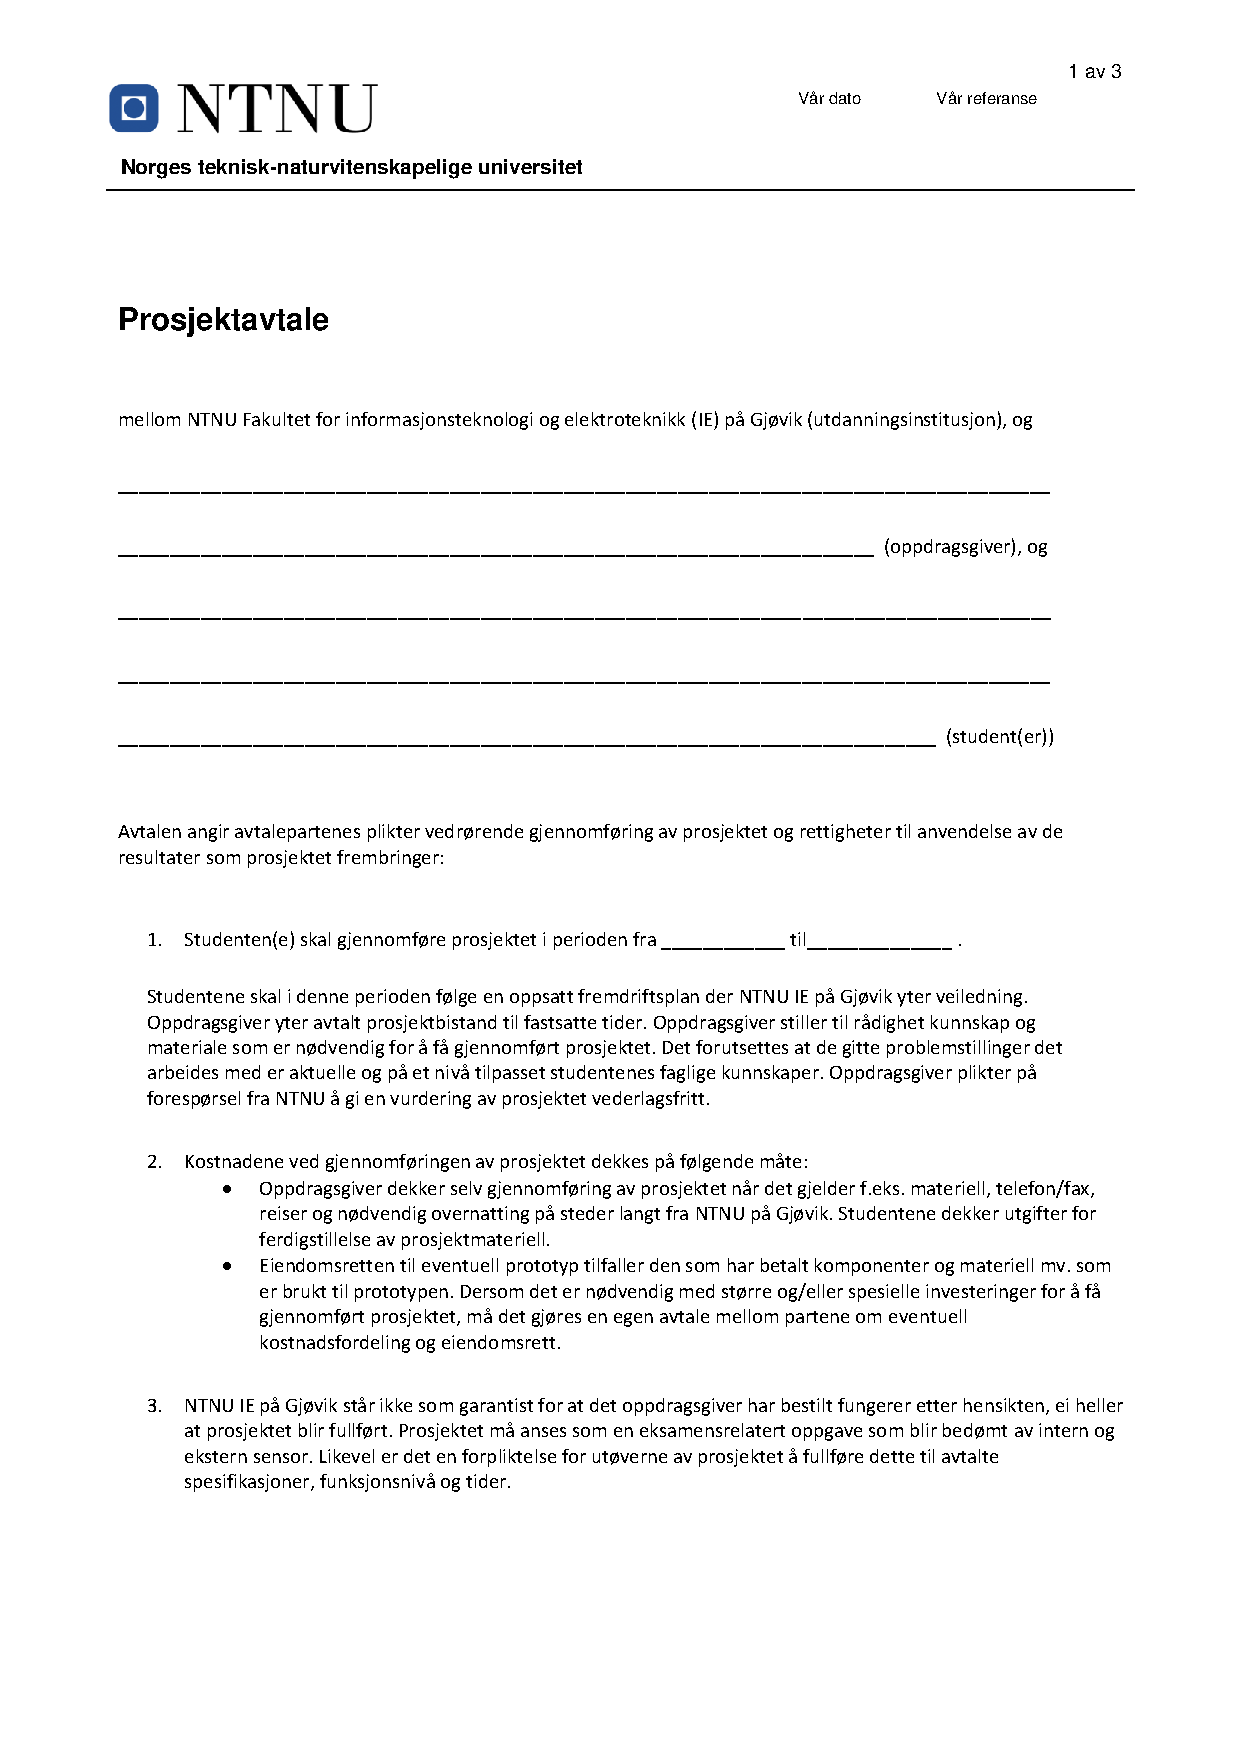
\includepdf[pages=-]{appendices/NTNUProsjektavtale.pdf}

\end{document}
